\documentclass[conference]{IEEEtran}
\usepackage{graphicx}
\usepackage{amsmath}
\usepackage{amsfonts}
\usepackage{hyperref}
\begin{document}
\title{Neural and Gaussian Process Surrogates for Fast Monte Carlo VaR and CVaR Estimation}
\author{Anonymous}
\maketitle

\begin{abstract}
Value-at-Risk (VaR) and Conditional Value-at-Risk (CVaR) are fundamental risk measures in finance...
\end{abstract}

\section{Introduction}
... See Figure~\ref{fig:ground_truth}.

\begin{figure}[!t]
  \centering
  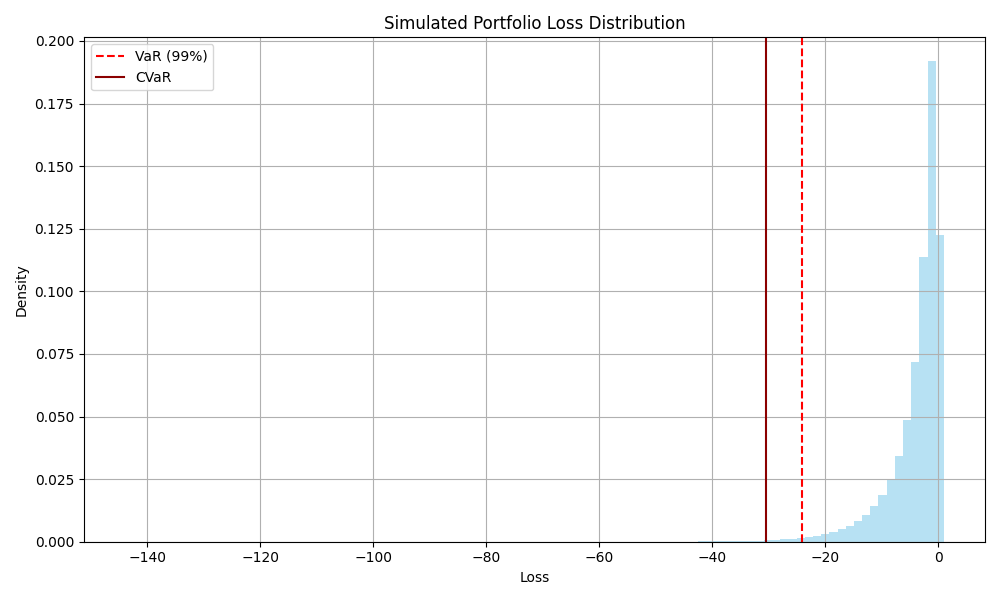
\includegraphics[width=\linewidth]{ground_truth.png}
  \caption{Ground-truth distribution of portfolio losses.}
  \label{fig:ground_truth}
\end{figure}

\section{Methodology}
\begin{figure}[!t]
  \centering
  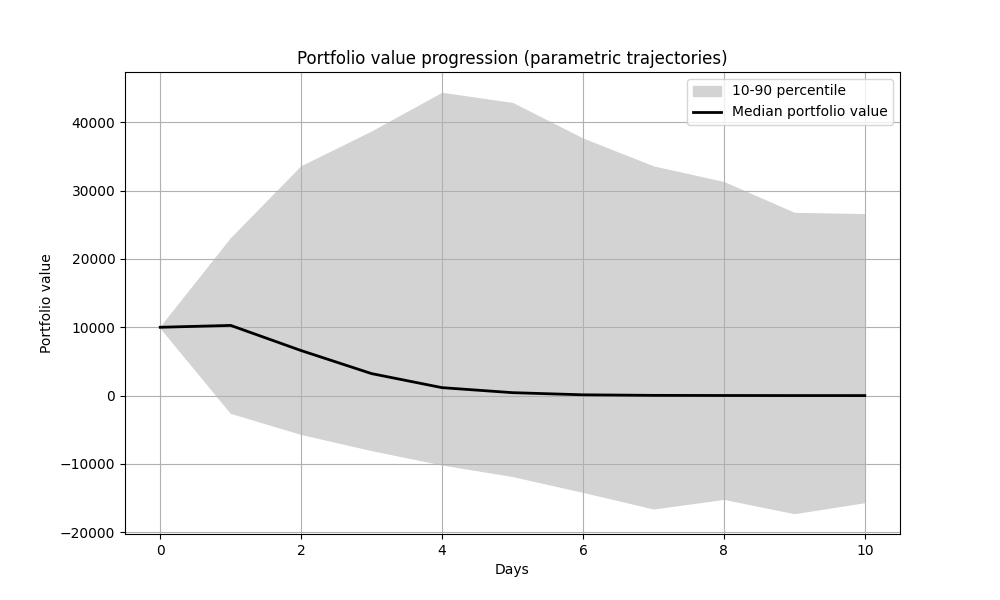
\includegraphics[width=\linewidth]{portfolio_projection.png}
  \caption{2D projection of scenario space with loss coloring.}
  \label{fig:portfolio_projection}
\end{figure}

\begin{figure}[!t]
  \centering
  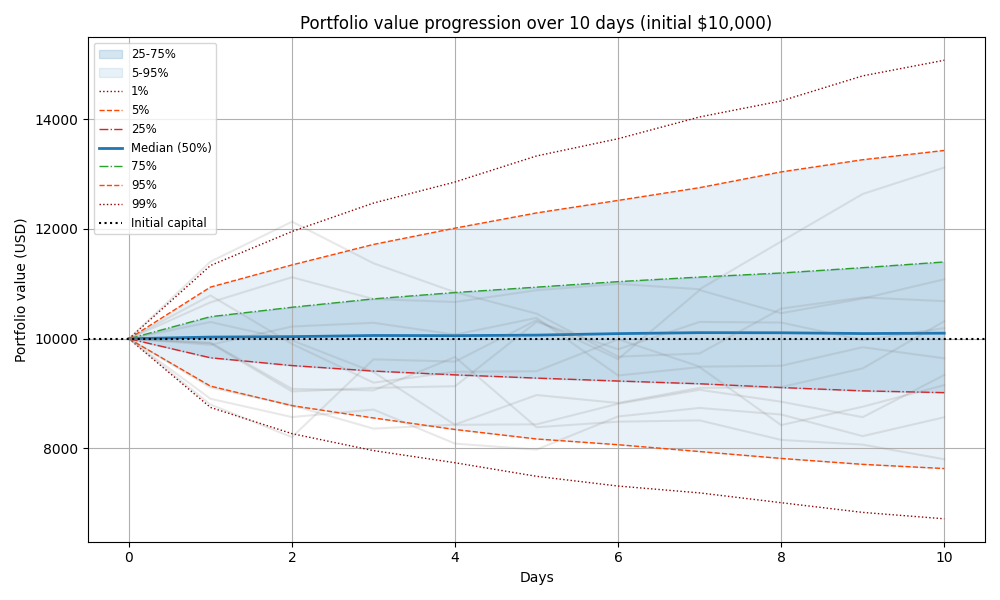
\includegraphics[width=\linewidth]{portfolio_value.png}
  \caption{Loss histogram in training set.}
  \label{fig:portfolio_value}
\end{figure}

\begin{figure}[!t]
  \centering
  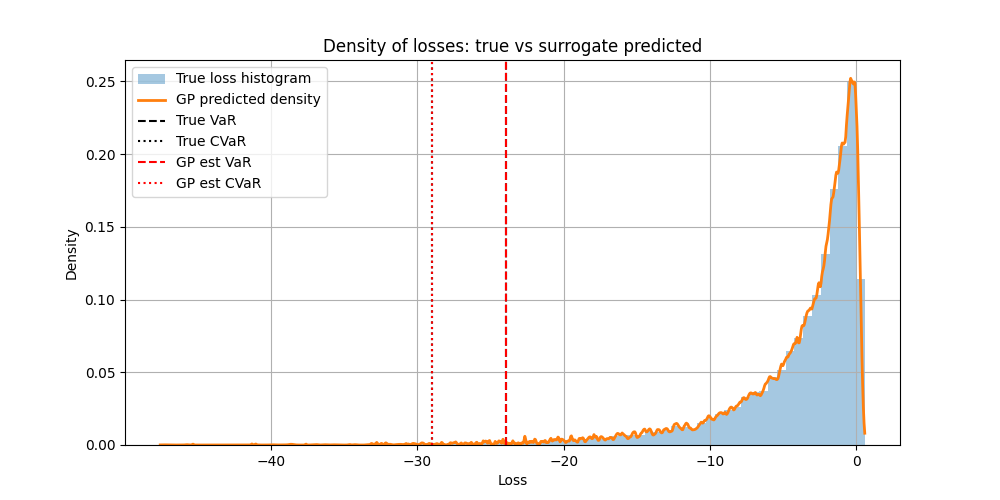
\includegraphics[width=\linewidth]{100m_gp_predicted_portfolio.png}
  \caption{GP surrogate loss distribution.}
  \label{fig:gp_pred}
\end{figure}

\begin{figure}[!t]
  \centering
  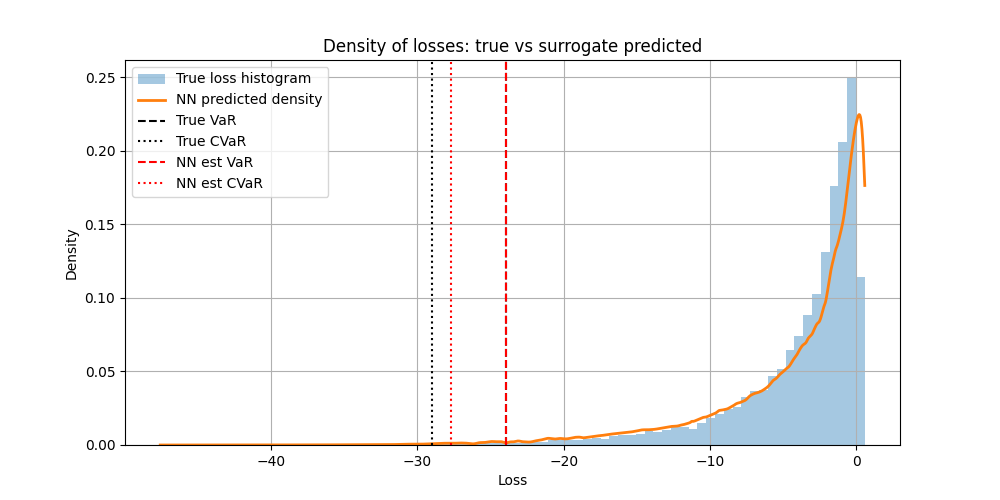
\includegraphics[width=\linewidth]{100m_nn_predicted_portfolio.png}
  \caption{NN surrogate loss distribution.}
  \label{fig:nn_pred}
\end{figure}

\begin{figure}[!t]
  \centering
  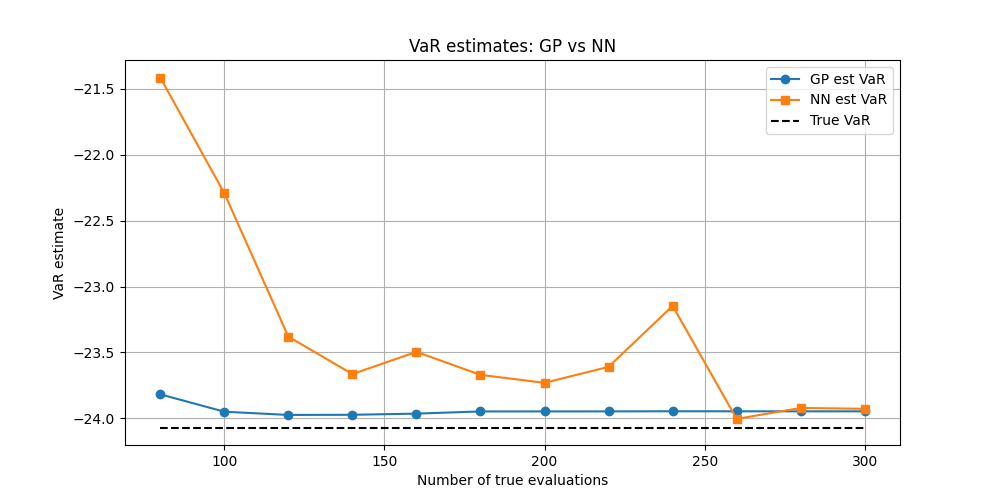
\includegraphics[width=\linewidth]{100m_var_comparison.png}
  \caption{VaR estimates: Surrogates vs Monte Carlo.}
  \label{fig:var_comp}
\end{figure}

\begin{figure}[!t]
  \centering
  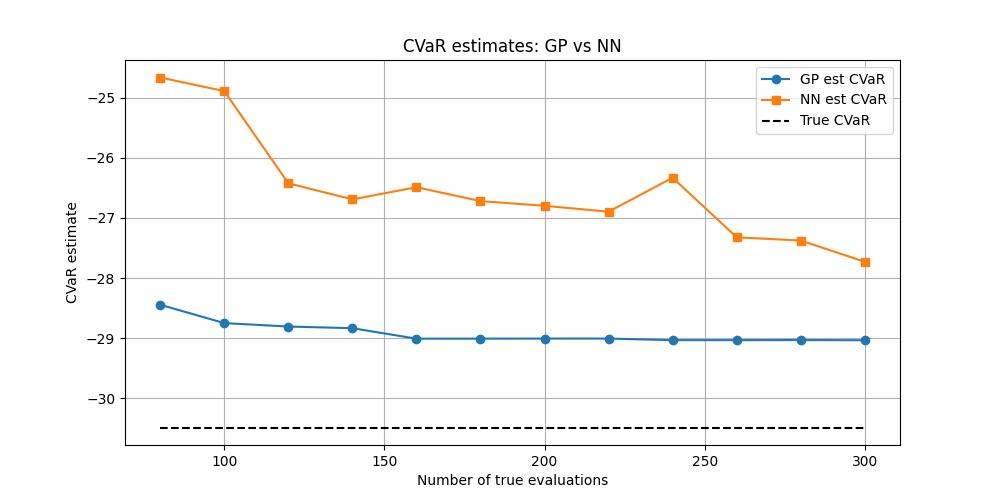
\includegraphics[width=\linewidth]{100m_cvar_comparison.png}
  \caption{CVaR estimates: Surrogates vs Monte Carlo.}
  \label{fig:cvar_comp}
\end{figure}

\begin{figure}[!t]
  \centering
  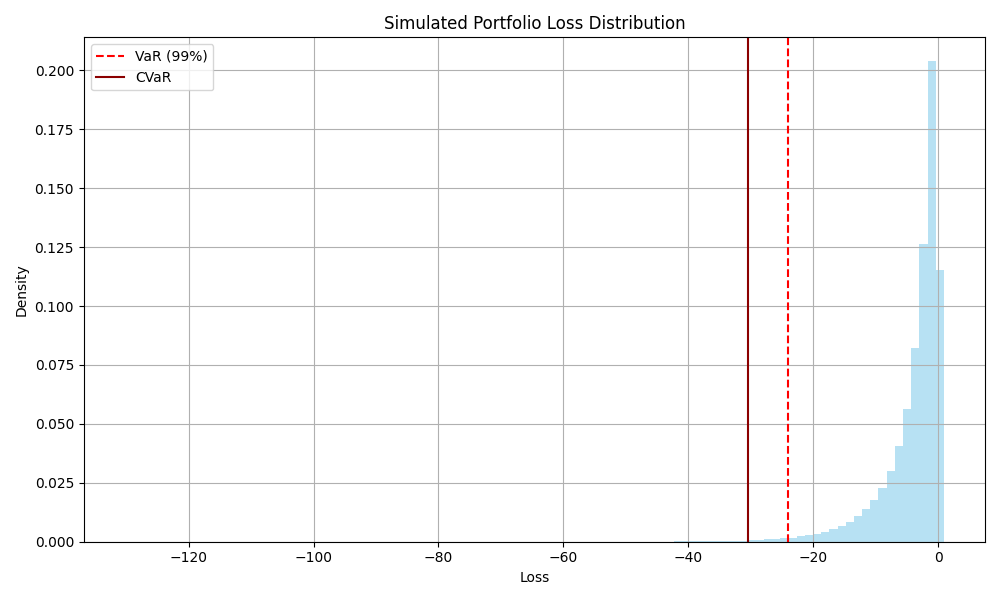
\includegraphics[width=\linewidth]{100m_Var_cvar.png}
  \caption{Surrogate-predicted vs True VaR/CVaR.}
  \label{fig:vc_comp}
\end{figure}

\bibliographystyle{IEEEtran}
\begin{thebibliography}{1}
\bibitem{glasserman2000efficient}
P.~Glasserman et al., ``Efficient Monte Carlo methods for value-at-risk,'' \emph{J. Risk}, vol.~2, 2000.

\bibitem{rockafellar2000optimization}
R.~T. Rockafellar and S.~Uryasev, ``Optimization of conditional value-at-risk,'' \emph{Financial Eng. News}, vol.~14, 2000.

\bibitem{surrogatemodel}
``Surrogate model,'' Wikipedia, 2025. [Online]. Available: \url{https://en.wikipedia.org/wiki/Surrogate_model}
\end{thebibliography}

\end{document}
